\chapter{Modélisation de systèmes}

Ce dernier chapitre couvrira la modélisation des comportements d'un système. La modélisation d'un système se fait dans les premières étapes de l'analyse et a pour but d'expliquer les objectifs du système, ses interactions et ses états. La modélisation du système répond aux questions «~quoi~» et «~qui~», laissant le «~comment~» à d'autres étapes. Elle demande de couvrir plusieurs aspects dont :

\begin{enumerate}
	\item La relation des entités actrices avec les cas d'utilisation;
	\item La relation des entités actrices avec le système dans l'exécution d'un cas d'utilisation particulier;
	\item Les relations entre les objets du domaine;
	\item Les états des objets du système dans l'exécution du système;
	\item Les états d'un objet dans l'exécution d'un cas d'utilisation.
\end{enumerate} 

La section \fullref{sec:cas-utilisation} décrit le premier aspect, soit la relation des entités actrices \index{Diagramme des cas d'utilisation!entite actrice} avec les cas d'utilisation, en utilisant les diagrammes des cas d'utilisation \index{Diagramme des cas d'utilisation}. La seconde section, \fullref{sec:dss}, présente le second aspect soit les \index{Diagramme de séquence système} interactions entre une entité actrice et le système dans un scénario donné. \\

Les trois autres aspects de la modélisation ne sont pas explicitement traités dans ce guide, mais correspondent à des cas particuliers de diagrammes précédemment couverts. La représentation des objets du domaine peut se faire avec un diagramme de classe (voir\fullref{sec:dc}) et la modélisation des états d'un objet dans un système ou dans l'exécution d'un cas d'utilisation peut se faire avec un diagramme d'états-transitions adapté (voir \fullref{sec:det}).\\

Il faut se rappeler que l'\gls{artefact} le plus important de la modélisation d'un système est le texte du document d'analyse. Les diagrammes offrent des représentations intéressantes du système qui facilitent la compréhension de certains aspects, mais qui ne permettent pas d'aller aussi en profondeur que ne le fait la description détaillée du système.

\secdiagramme{Diagramme des cas d'utilisation}{Analyse}{UML 2.5}{Use case diagram}
\label{sec:cas-utilisation}

Un \gls{diag-cu} (\acrshort{DCU}) présente les \glspl{entite-actrice} du système et les relie aux \glspl{cas-utilisation} qu'ils peuvent réaliser. La base du diagramme est un grand rectangle qui représente le système en lui-même. Dans le rectangle, les différents cas d'utilisation sont placés dans des ovales. Le rectangle peut être omis, mais il est quand même suggéré de le représenter.

\begin{figure}[H]
	\caption{Représentation du système et des \acrshort{CU} dans un \acrshort{DCU}} 
	\centering
	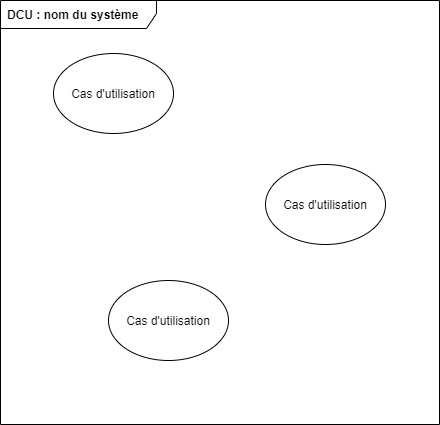
\includegraphics[width=.7\textwidth]{cas-utilisation1.png}
\end{figure}

Les entités actrices humaines sont représentées par des bonshommes allumettes situés de part et d'autre du système. La position des entité actrices est régie par les règles suivantes :

\begin{itemize}
	\item Les \term{\glspl{acteur-primaire}} sont situés à gauche du système;
	\item Les \term{\glspl{acteur-secondaire}} sont situés à droite du système.
	\item Les \term{\glspl{partie-prenante}} ne sont pas représentées, car elles ne réalisent pas de \glspl{CU}.
\end{itemize}

\vfill

\begin{figure}[H]
	\caption{Représentation des acteurs dans un \acrshort{DCU}} 
	\centering
	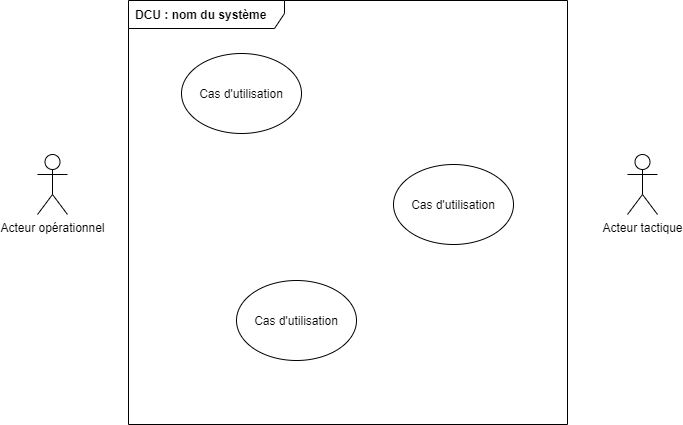
\includegraphics[width=.85\textwidth]{cas-utilisation2.png}
\end{figure}

Lorsqu'une entité actrice peut réaliser l'un des cas d'utilisation, un trait plein relie l'entité actrice et le \gls{cas-utilisation}. Un même cas d'utilisation peut être associé à plusieurs entités actrices s'il peut être réalisé par plusieurs d'entre elles. \\

On retrouve aussi une relation d'\gls{heritage-acteur} \index{Diagramme des cas d'utilisation!héritage d'acteurs} qui signifie qu'un acteur (enfant) peut exécuter tous les cas d'utilisation d'un autre acteur (parent). Cette relation est représentée par une flèche avec une tête vide qui part de l'entité enfant vers l'entité parent.

\begin{figure}[H]
	\caption{Flèche d'héritage d'acteur}
	\centering
	
\includegraphics[scale=0.4]{fleche-heritage.png}
\end{figure}

\begin{exemple}[label={ex:acteurs-cu}]{Acteurs et CU entre \acrshort{CU}}
	Dans la modélisation (partielle) d'un système de gestion d'école (semblable au système {\itshape Omnivox}), on retrouve les CU suivants :
	\begin{itemize}
		\item Ajouter une nouvelle évaluation;
		\item Remettre une évaluation;
		\item Saisir les résultats d'une évaluation;
		\item Consulter les notes pour un cours;
		\item Gérer les accès.
	\end{itemize}
	On retrouve aussi les acteurs suivants :
	\begin{itemize}
		\item Personne étudiante;
		\item Personne enseignante;
		\item Responsable de la coordination départementale (qui est une personne enseignante);
		\item Personne administrant le système.
	\end{itemize}
	
	\begin{center} 
		\captionof{figure}{Exemple d'acteurs et de cas d'utilisation}
		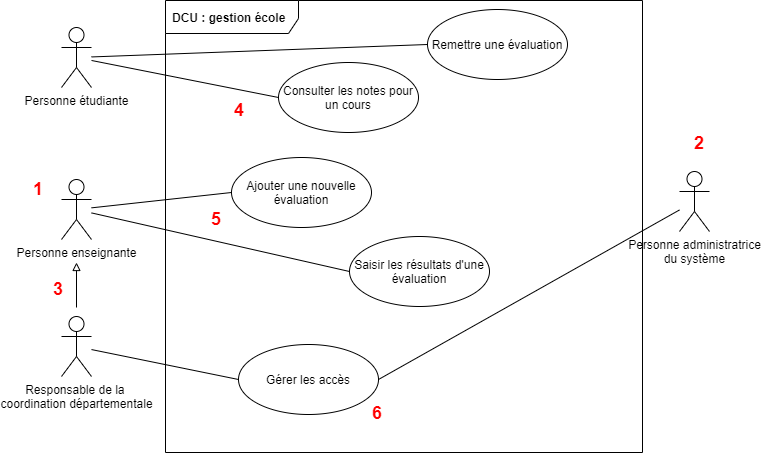
\includegraphics[width=.95\textwidth]{cas-utilisation-Exemple acteurs et CU.drawio.png}
	\end{center}
	
	Sur le précédent diagramme, on peut observer les éléments suivants :
	
	\begin{enumerate}
		\item Les personnes étudiantes, personnes enseignantes et personnes responsables de la coordination départementale sont des acteurs opérationnels (primaires). Les personnages qui les représentent sont à gauche de la boîte qui symbolise le système. 
		\item Les personnes administrant le système sont des acteurs tactiques (secondaires). Ils sont représentés à droite de la boîte qui symbolise le système.
		\item La personne responsable de la coordination départementale \term{hérite} de l'acteur «~personne enseignante~», car il s'agit d'une personne enseignante avec des responsabilités supplémentaires.
		\item Les personnes étudiantes peuvent remettre une évaluation et consulter les notes pour un cours qu'elles suivent.
		\item Les personnes enseignantes peuvent ajouter une nouvelle évaluation ou saisir les résultats d'une évaluation.
		\item Les personnes responsables de la coordination départementale et les personnes administrant le système peuvent toutes deux gérer les accès. Si l'exécution du cas prévoit des droits différents dans la gestion des rôles, cette différence est explicitée au niveau des descriptions des cas.
	\end{enumerate}
	
\end{exemple}

\subsection{Relations entre cas d'utilisation}

Les cas d'utilisations peuvent être liés entre eux par deux types de relations. Ces relations sont :

\begin{itemize}
	\item \term{\Gls{extend}} \index{Diagramme des cas d'utilisation!extend} : indique que le comportement d'un cas d'utilisation peut être étendu par un autre cas d'utilisation. L'endroit où l'extension peut se produire est présenté par des \term{\glspl{point-extension}}. \index{Diagramme des cas d'utilisation!points d'extension} Le \acrshort{CU} dont le comportement est modifié ne sait pas que son comportement est modifié.
	\item \term{\Gls{include}} \index{Diagramme des cas d'utilisation!include} : indique que la réalisation d'un cas d'utilisation peut demander la réalisation d'un autre \acrshort{CU}. La description du \acrshort{CU} qui en inclut un autre spécifie les conditions de réalisation.
\end{itemize}

Les cas d'utilisation peuvent définir des \term{\glspl{point-extension}} qui sont des opérations (étapes) du \acrshort{CU} auxquelles il est possible d'ajouter plus de scénarios alternatifs que ce qui est précisé dans la description du cas d'utilisation.

On peut utiliser la relation \term{\gls{include}} dans deux contextes :
\begin{enumerate}
	\item Une opération est commune à plusieurs \acrshort{CU} : on déplace cette opération dans un nouveau \acrshort{CU} et chacun des \acrshort{CU} qui l'utilisent \term{\gls{include}} le nouveau \acrshort{CU}.
	\item Un \acrshort{CU} est très complexe, alors on le décompose en plus petits \acrshort{CU} et il \term{\gls{include}} chacune des parties créées. 
\end{enumerate}

\begin{figure}[H]
	\caption{Mise en œuvre des relations \term{\gls{include}} et \term{\gls{extend}}}
	\centering
	\begin{subfigure}[b]{0.45\textwidth}
		\centering
		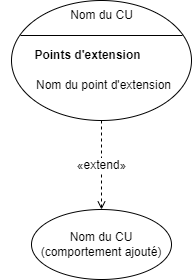
\includegraphics[scale=0.6]{relation extend.png}
		\caption*{Relation \term{\gls{extend}}}
	\end{subfigure} \hfill
	\begin{subfigure}[b]{0.45\textwidth}
		\centering
		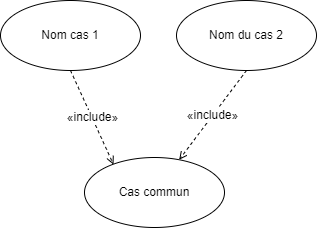
\includegraphics[scale=0.6]{relation include 2.png}
		\caption*{Relation \term{\gls{include}} (extraction d'un comportement commun)}
	\end{subfigure} \\
	~
	\hfill
	\begin{subfigure}[b]{0.6\textwidth}
		\centering
		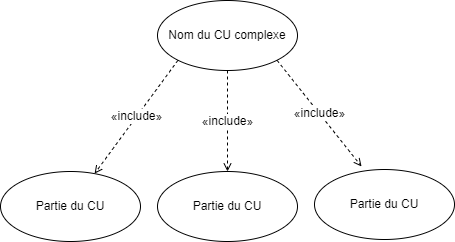
\includegraphics[scale=0.6]{relation include 1.png}
		\caption*{Relation \term{\gls{include}} (séparation d'un \acrshort{CU} complexe)}
	\end{subfigure}
	\hfill
	~
\end{figure}

\begin{bonnepratique}
	L'utilisation des relations, en particulier \term{include}, permet de simplifier l'écriture des descriptions des \acrshort{CU}. Cependant, une utilisation trop importante de ces relations sur le \acrshort{DCU} risque d'en diminuer la lisibilité et donc l'utilité.\\
	
	Il faut donc, lorsqu'on prépare le \acrshort{DCU}, se limiter à illustrer uniquement les relations qui apportent une information supplémentaire significative. Par exemple, indiquer qu'un \acrshort{CU} qui traite des {\itshape paiements} inclus le \acrshort{CU} de {\itshape  paiement par carte de crédit} est tout à fait adéquat. Par contre, indiquer pour 80\% des \acrshort{CU} qu'ils incluent comme opération préalable le \acrshort{CU} de {\itshape vérifier l'authentification} alourdit grandement la notation sans apporter de nouvelle information significative et est, par conséquent, une pratique à éviter.
\end{bonnepratique}

\begin{distinction}{la relation \term{\gls{include}}}{la relation \term{\gls{extend}}}
	
	{\em Pareil} : la relation \term{\gls{include}} et la relation \term{\gls{extend}} servent toutes deux à représenter la possibilité de réaliser un \acrshort{CU} dans un autre \acrshort{CU}. \\
	
	{\em Différent } : dans la relation \term{\gls{include}}, la description du \acrshort{CU} qui en inclut un autre précise dans quelles conditions le cas inclus se réalise. La relation \term{\gls{extend}} le \acrshort{CU} inclut se greffe au cas principal par un des \term{\glspl{point-extension}} du \acrshort{CU} principal. La description du cas principal ne précise pas quand le \acrshort{CU} inclus se réalise.   
\end{distinction}

\begin{exemple}{Relations entre \acrshort{CU}}
	Dans la modélisation d'un système de gestion d'école tel que présenté à l'exemple~\ref{ex:acteurs-cu}, on peut utiliser la relation \term{\gls{include}} dans la situation suivante :
	
	\begin{enumerate}
		\item Envoyer un message lorsqu'un nouveau travail ou une nouvelle note d'évaluation est disponible. Comme les deux \acrshort{CU} réalisent la même opération, on peut donc la définir dans un \acrshort{CU} qui lui est propre. 
	\end{enumerate}
	
	On peut utiliser la relation \term{\gls{extend}} dans la situation suivante :
	
	\begin{enumerate}
		\setcounter{enumi}{1}
		\item Ajouter une ressource à une évaluation. Comme on ne peut pas définir tous les types de documents ou ressources que l'on peut joindre à une évaluation  (document word, excel, powerpoint, pdf..., on peut ouvrir le cas «~Ajouter une évaluation~» en lui définissant le point d'extension «~Ajouter une ressource~». Par la suite, on pourra définir un cas d'utilisation pour chaque type de ressource que l'on trouvera pertinent de joindre à une évaluation. L'ajout de nouveau type de ressource ne modifiera pas le cas de base d'«~Ajouter une évaluation~».
	\end{enumerate}
	
	\pagebreak
	
	\begin{center} 
		\captionof{figure}{Mise en œuvre des relations \term{\gls{include}} et \term{\gls{extend}} }
		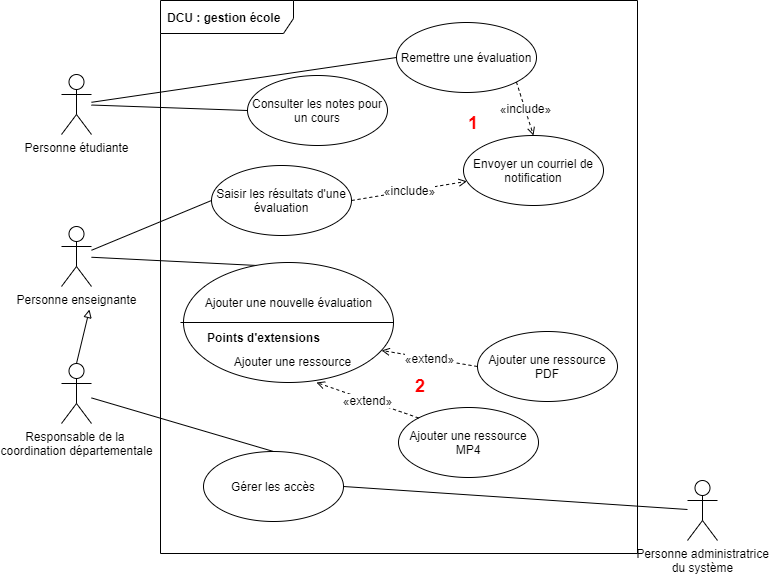
\includegraphics[width=.95\textwidth]{cas-utilisation-Exemple include et extend.drawio.png}
	\end{center} 
	
\end{exemple}

\subsection{Banque de dépannage}

\question{Mon diagramme ressemble à un spaghetti. Que puis-je faire ?}

\begin{itemize}
	\item[$\mathbf{\star}$] Enlever les relations inutiles. Un \term{\gls{include}} ou un \term{\gls{extend}} qui permet d'inclure un seul autre cas particulier peut être simplifié et intégré directement dans la description du \acrshort{CU}.
	\item[$\mathbf{\star}$] Enlever des informations redondantes ou qui n'ont pas un apport significatif à la compréhension de la structure du système. Si un grand nombre de \acrshort{CU} ont tous une relation de type \term{\gls{include}} qui pointe vers le même \acrshort{CU} (par exemple, 20 \acrshort{CU} demandent d'être préalablement authentifiés), il n'est pas très pertinent d'indiquer ces relations sur le diagramme. On peut simplement prendre la section des \term{\glspl{precondition}} \index{Diagramme des cas d'utilisation!précondition} ou des \term{\glspl{postcondition}} \index{Diagramme des cas d'utilisation!postcondition} pour indiquer l'information. Dans le cas d'une gestion d'erreur, on peut simplement omettre l'information sur le diagramme et l'indiquer comme \term{\gls{scenario-exception}} dans la description de chaque \acrshort{CU}.
	\item Réorganiser les acteurs afin de les rapprocher des cas d'utilisation qui leur sont associés.
	\item Vérifier s'il y a une relation d'héritage entre des acteurs et utiliser cette relation pour représenter moins de liens sur le diagramme.
\end{itemize}

\question{Je ne sais pas si je dois utiliser \term{\gls{include}} ou \term{\gls{extend}}}

\begin{itemize}
	\item[$\mathbf{\star}$] Si vous pouvez indiquer dans quelles conditions le cas se réalise, alors il s'agit probablement d'un \term{\gls{include}}, autrement il s'agit probablement d'un \term{\gls{extend}}.
\end{itemize}

\question{J'ai terminé mon diagramme et j'ai presque pas / aucune relation \term{\gls{include}} ou \term{\gls{extend}}. Est-ce correct ?}

\begin{itemize}
	\item[$\mathbf{\star}$] Oui, les relations entre \acrshort{CU} sont relativement rares et chercher à en créer artificiellement amène souvent à s'éloigner du besoin réel du client. Le principal effort de la description d'un système se fait dans la description textuelle des \acrshort{CU} et non dans l'élaboration du \gls{diag-cu}. 
\end{itemize}

\secdiagramme{Diagramme de séquence système}{Analyse}{UML 2.5}{System sequence diagram, Sequence diagram}
\label{sec:dss}

Dans la description détaillée des \glspl{cas-utilisation}, on retrouve une description textuelle des messages entre les acteurs, le système et les sous-systèmes. Il peut être utile de modéliser graphiquement le séquençage de ces opérations afin d'obtenir une meilleure vue d'ensemble sur la circulation des informations entre les acteurs et le système. C'est ce que l'on appelle les \glspl{diag-seq-sys} \acrshort{DSS} \index{Diagramme de séquence système}. La syntaxe de ces diagrammes ressemble à celle des diagramme de séquence \fullref{arg1}. \\

\begin{important}
	Il faut se rappeler que le but d'un \acrshort{DSS} n'est pas de remplacer la description textuelle d'un CU, mais bien de faciliter la compréhension du CU en fournissant une vue d'ensemble des opérations clés.
\end{important}

Dans cette modélisation, on considère que le système agit selon un principe appelé la \gls{boite-noire}. On représente donc uniquement les commandes passées aux systèmes, les données entrantes et les messages retournés par le système. Cette modélisation est souvent très proche de la description textuelle du cas, mais permet d'obtenir une vue d'ensemble des messages du système.

\begin{distinction}{diagramme de séquence}{diagramme de séquence système}
	Il existe deux situations où les diagrammes de séquence peuvent être utilisés, et dans les deux cas, la notation est la même. Afin de différencier les deux types de diagrammes, l'appellation \gls{diag-seq} fait référence au diagramme qui présente le séquençage des appels entre des objets du système. Le \gls{diag-seq-sys} présente le séquençage des appels entre les acteurs et le système. C'est ce deuxième type qui est présenté dans cette section.
\end{distinction}

\subsection{Acteurs, système et sous-système}

Les entités qui participent à la réalisation des cas d'utilisation sont représentées sous forme d'un trait pointillé auquel les messages qu'ils émettent ou reçoivent viennent s'accrocher. Les systèmes et sous-systèmes sont identifiés par une boîte, alors que les acteurs sont identifiés par des bonshommes allumettes. Sous chaque élément est tracé une ligne appelée «~ligne d'instance~» (on utilise souvent le terme «~ligne de vie~», même si ce dernier est incorrect) en pointillé de laquelle provient ou s'y termine les messages qui impliquent l'élément. Le nom de l'entité est précédé du symbole deux points «~:~».\\

On présente les éléments dans l'ordre suivant sur un \acrshort{DSS}:
\begin{enumerate}
	\item À gauche complètement on retrouve l'\term{acteur principal} du scénario représenté;
	\item Immédiatement à la droite de l'acteur principal on retourne le \term{système};
	\item On retrouve ensuite, en ordre d'appel, de la gauche vers la droite, les \term{sous-systèmes} et les \term{acteurs secondaires}.
\end{enumerate}

\begin{figure}[H]
	\caption{Élément et lignes d'instances des \acrshort{DSS}}
	\centering
	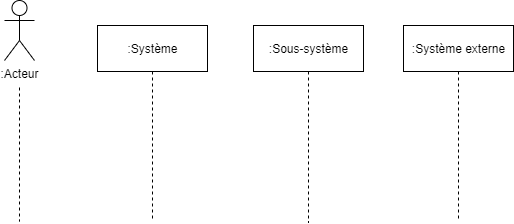
\includegraphics[scale=0.6]{dss-element.png}
\end{figure}

\subsection{Messages}

Différents messages peuvent circuler entre les acteurs et les systèmes. Les messages des acteurs vers le système prennent la forme d'une flèche pleine sur laquelle le nom du message est écrit. Les réponses du système vers les acteurs prennent la forme d'une flèche pointillée avec la ou les valeurs retour inscrites sur la flèche. Les messages sont nommés avec une terminologie informelle (qui n'est pas liée à un langage de programmation).\\

Si le message comporte des paramètres, ceux-ci sont indiqués entre parenthèses, toujours en utilisant une terminologie informelle. S'il y a plusieurs paramètres, ils sont séparés par une virgule. Si un message ne donne pas lieu à une réponse, la flèche de réponse est omise.

\begin{figure}[H]
	\caption{Messages entre un acteur et le système}
	\centering
	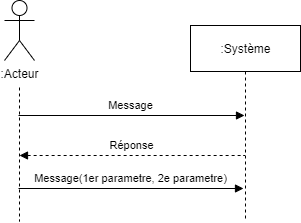
\includegraphics[scale=0.6]{dss-messages.png}
\end{figure}

\begin{exemple}[label={ex:modelisation-cu-1}]{Modélisation du CU «~Remettre une évaluation~» }
	Reprenons la situation définie à l'exemple \ref{ex:acteurs-cu} où l'on modélise un système de gestion d'établissement scolaire semblable au système {\itshape Omnivox}. Le cas modélisé est celui où une personne étudiante remet une évaluation. \\
	
	{\bfseries \Large Nom du CU : Remettre une évaluation}\\[6pt]
	{\bfseries Acteur principal : } personne étudiante\\[6pt]
	{\bfseries Préconditions : }
	\begin{itemize}
		\item La personne étudiante est connectée au système.
		\item La personne étudiante a été assignée à au moins un travail.
		\item La personne étudiante possède un document qu'elle veut remettre.
	\end{itemize} 
	{\bfseries Scénario principal}
	\begin{enumerate}
		\item La personne étudiante sélectionne le travail qu'elle souhaite remettre parmi les travaux qui lui sont assignés.
		\item Le système affiche un formulaire de remise de travail.
		\item La personne étudiante sélectionne le fichier à remettre.
		\item Le système confirme le téléversement complet du fichier.
		\item La personne confirme la remise du travail.
		\item Le système informe le sous-système de messagerie d'envoyer une confirmation de remise à la personne étudiante.
		\item Le système confirme l'enregistrement de la remise.
	\end{enumerate}
	{\bfseries Postconditions : }
	\begin{itemize}
		\item Un fichier a bien été téléversé dans le système.
		\item Un courriel de confirmation a été envoyé à la personne étudiante.
	\end{itemize} 
	
	Voici le \gls{DSS} relatif à ce cas d'utilisation.
	
	\pagebreak
	
	\begin{center} 
		\captionof{figure}{Modélisation du cas d'utilisation par \acrshort{DSS}} 
		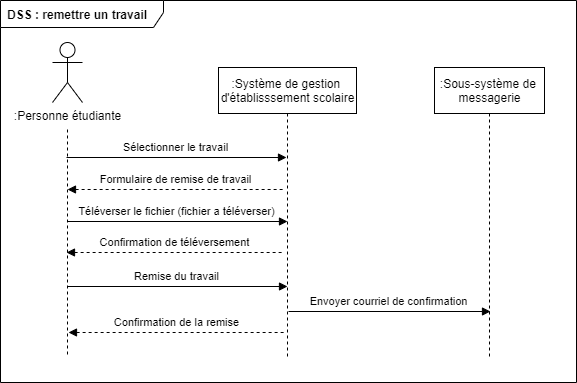
\includegraphics[width=.95\textwidth]{dss-Exemple-simple.png}
	\end{center}  
\end{exemple}

\subsection{Blocs}

On peut tenir compte des scénarios d'extension et des opérations conditionnelles ou répétées à l'aide des blocs. Il existe 3 types de blocs :~\term{optionnel}, \term{traitement répétitif} et \term{alternatif}. Chaque bloc prend la forme d'un encadré avec une vignette d'information en haut à gauche qui renseigne sur son type. Chaque bloc peut être accompagné d'une paire de crochets pour indiquer des informations spécifiques à la situation.\\

Les messages qui sont envoyés de façon conditionnelle ou répétée sont dans le bloc. Si le bloc contient plusieurs zones, celles-ci sont séparées par une ligne pointillée.

\begin{figure}[H]
	\caption{Blocs dans les \glspl{diag-seq}}
	\centering
	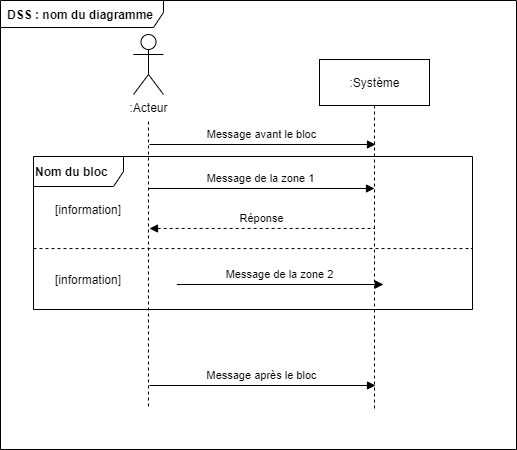
\includegraphics[scale=0.6]{dss-blocs.png}
\end{figure}

\begin{enumerate}
	\item Le bloc \term{optionnel} permet de gérer la présence de conditions de garde \index{Condition de garde} dans le code. Le bloc est composé d'une seule zone avec une condition de garde. Le code dans le bloc est exécuté si la condition de garde est vraie.
	\item Le bloc \term{répétitif} permet de gérer des opérations répétées tant qu'une condition est vraie. Le bloc contient une seule zone d'instructions à répéter.
	\item Le bloc \term{alternatif} permet de gérer plusieurs conditions quelconques et exclusives. Seul le code dans le bloc où la condition est vérifiée sera exécuté.
\end{enumerate}

\begin{figure}[H]
	\caption{Différents types de blocs de traitement dans les \acrshort{DSS}}
	\centering
	\begin{minipage}[b]{.48\textwidth}
		\begin{subfigure}[b]{.45\textwidth}
			\centering
			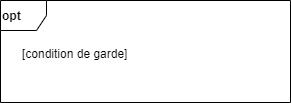
\includegraphics[scale=0.7]{dss-bloc-opt.png}
			\caption*{Bloc \term{optionnel}}
		\end{subfigure} \\
		\begin{subfigure}[b]{0.45\textwidth}
			\centering
			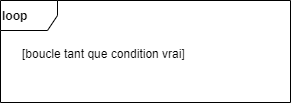
\includegraphics[scale=0.7]{dss-bloc-loop.png}
			\caption*{Bloc \term{répétitif}}
		\end{subfigure}
	\end{minipage}
	\hfill
	\begin{minipage}[b]{.48\textwidth}
		\vfill
		\begin{subfigure}[b]{0.45\textwidth}
			\centering
			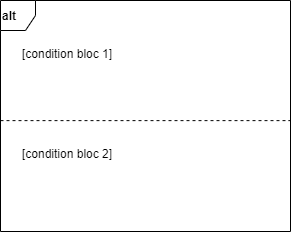
\includegraphics[scale=0.7]{dss-bloc-alt.png}
			\caption*{Bloc \term{alternatif}}
		\end{subfigure}
		\vfill
	\end{minipage}
\end{figure}

\begin{exemple}{Modélisation du CU «~Remettre une évaluation~» avec les blocs de traitement}
	Reprenons l'exemple \ref{ex:modelisation-cu-1} et bonifions la description du cas d'utilisation. Le cas modélisé est celui où une personne étudiante remet une évaluation. Les étapes ajoutées sont inscrites en rouge.  \\
	
	{\bfseries \Large Nom du CU : Remettre une évaluation}\\[6pt]
	{\bfseries Acteur principal : } personne étudiante\\[6pt]
	{\bfseries Préconditions : }
	\begin{itemize}
		\item La personne étudiante est connectée au système.
		\item La personne étudiante a été assignée à au moins un travail.
		\item La personne étudiante possède un document qu'elle veut remettre.
	\end{itemize} 
	{\bfseries Scénario principal}
	\begin{enumerate}
		\item La personne étudiante sélectionne le travail qu'elle souhaite remettre parmi les travaux qui lui sont assignés.
		\item Le système affiche un formulaire de remise de travail.
		\item La personne étudiante sélectionne le fichier à remettre.
		\item Le système confirme le téléversement complet du fichier.
		\reditem La personne étudiante répète l'étape 3 pour chaque fichier supplémentaire à remettre.
		\reditem La personne étudiante coche la case qui atteste qu'elle a produit elle-même le travail et qu'elle a cité les sources utilisées adéquatement.
		\item La personne confirme la remise du travail.
		\item Le système informe le sous-système de messagerie d'envoyer une confirmation de remise à la personne étudiante.
		\item Le système confirme l'enregistrement de la remise.
	\end{enumerate}
	{\bfseries Postconditions : }
	\begin{itemize}
		\item Un fichier a bien été téléversé dans le système.
		\item Un courriel de confirmation a été envoyé à la personne étudiante.
	\end{itemize} 
	{\color{red} \bfseries Scénario d'extension : }
	\begin{itemize}
		\reditem[6a] La personne étudiante souhaite lire la politique de plagiat 
		\begin{enumerate}
			\reditem La personne étudiante clique sur le lien pour lire la politique de plagiat.
			\reditem Le système affiche la politique de plagiat. 
		\end{enumerate}
	\end{itemize}
	
	Voici le \gls{DSS} relatif à ce cas d'utilisation.
	
	\pagebreak
	
	\begin{center} 
		\captionof{figure}{Modélisation du cas d'utilisation par \acrshort{DSS}} 
		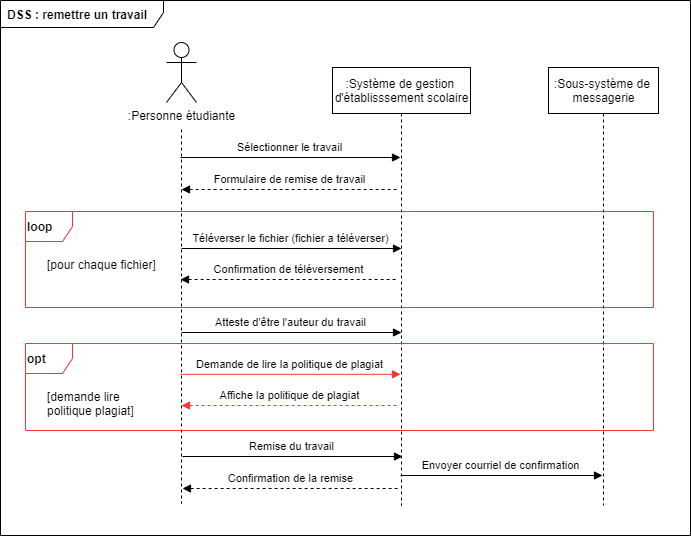
\includegraphics[width=.95\textwidth]{dss-Exemple-complet.png}
	\end{center}  
\end{exemple}

\subsection{\Glspl{precondition} et \glspl{postcondition}}

On peut représenter les \glspl{precondition} et les \glspl{postcondition} sur un \acrshort{DSS} avec une boîte aux coins arrondis située sur la ligne d'instance de l'entité à laquelle la condition s'applique. La présence des \glspl{precondition} et des \glspl{postcondition} est toutefois optionnelle. Il faut éviter de surcharger le diagramme, donc elles sont souvent omises lorsqu'elles sont nombreuses.

\begin{figure}
	\caption{Représentation des \glspl{precondition} et des \glspl{postcondition} sur un \acrshort{DSS}}
	\centering
	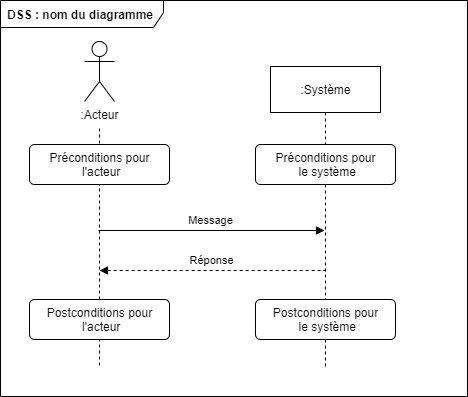
\includegraphics[scale=0.6]{dss-pre-post.png}
\end{figure}

\FloatBarrier

\subsection{Commentaires}

Pour apporter des précisions supplémentaires sur le diagramme, on peut utiliser des commentaires. Ceux-ci prennent la forme de rectangle avec un coin replié. Une ligne pointillée pointe sur l'élément du diagramme auquel le commentaire s'applique. Si le commentaire ne vise pas un élément particulier, la ligne est omise. Il est important de limiter les commentaires afin de ne pas saturer le diagramme.

\begin{figure}
	\caption{Représentation des commentaires sur un \acrshort{DSS}}
	\centering
	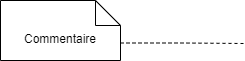
\includegraphics[scale=0.6]{dss-commentaire.png}
\end{figure}

\FloatBarrier

\subsection{Exemples}

\subsection{Banque de dépannage}

\question{J'ai plusieurs entité actrices humaines sur mon diagramme, est-ce correct ?}

Peut-être que oui, peut-être que non. Le \acrshort{DSS} sert à indiquer des interactions entre le système et des entité actrices. Le risque à avoir plusieurs entités actrices humaines sur un même diagramme est de représenter les interactions entre les entités actrices. Deux éléments à observer pour répondre à cette question sont :
\begin{enumerate}
	\item Chaque entité actrice doit minimalement interagir {\bfseries directement} une fois avec le système indépendamment des autres acteurs. 
	\item Il ne doit pas y avoir de message allant d'une entité humaine vers une autre entité humaine.
\end{enumerate}

Il faut aussi noter qu'il est normal d'avoir plusieurs entité actrices sous-système dans un même \acrshort{DSS}. \\

\question{Est-ce que je dois représenter toutes les étapes du scénario principal, tous les scénarios d'extension et tous les scénarios d'exception sur mon \acrshort{DSS} ?}

Non, représenter toutes les étapes mène dans la plupart des cas à un diagramme surchargé et difficile à comprendre, ce qui est contraire à la raison même de faire un diagramme.\\

Normalement, toutes les étapes du scénario principal sont représentées, la majorité des extensions devraient l'être également. Les extensions complexes (plus de 5 étapes) pourraient faire l'objet d'un autre diagramme ou même d'un autre \acrshort{CU}.\\

Pour les extensions, on évite de représenter sur le \acrshort{DSS} celles qui :
\begin{itemize}
	\item Peuvent se produire à tout moment, car on ne peut pas les inclure à un endroit précis dans le diagramme.
	\item Provoque la fin du CU parce qu'il s'agit d'une erreur irrécupérable, car elles n'apportent pas d'information sur l'exécution du CU.
	\item Lié à une erreur d'entrée de donnée (comme un mauvais format de date), car elles ne changent pas le déroulement du CU.
\end{itemize}



